\chapter{Running the Solver \texttt{xspecfem3D}}\label{cha:Running-the-Solver}

Now that you have successfully run the mesher, you are ready to compile
the solver. For reasons of speed, the solver uses static memory allocation.
Therefore it needs to be recompiled (type `\texttt{make clean}' and
`\texttt{make specfem3D}') every time one reruns the mesher with different
parameters. To compile the solver one needs a file generated by the
mesher in the directory \texttt{OUTPUT\_FILES} called \texttt{values\_from\_mesher.h},
which contains parameters describing the static size of the arrays
as well as the setting of certain flags.\newline


The solver needs three input files in the \texttt{DATA} directory
to run: the \texttt{Par\_file} that was discussed in detail in Chapter~\ref{cha:Running-the-Mesher},
the earthquake source parameter file \texttt{CMTSOLUTION} or the force source parameter file {\texttt{FORCESOLUTION}}, and the
stations file \texttt{STATIONS}. Most parameters in the \texttt{Par\_file}
should be set prior to running the mesher. Only the following parameters
may be changed after running the mesher:\newline

\begin{itemize}
\item the simulation type control parameters: \texttt{SIMULATION\_TYPE}
and \texttt{SAVE\_FORWARD}
\item the record length \texttt{RECORD\_LENGTH\_IN\_MINUTES}
\item the movie control parameters \texttt{MOVIE\_SURFACE}, \texttt{MOVIE\_VOLUME},
and \texttt{NTSTEPS\_BETWEEN\_FRAMES}
\item the multi-stage simulation parameters \texttt{NUMBER\_OF\_RUNS} and
\texttt{NUMBER\_OF\_THIS\_RUN}
\item the output information parameters \texttt{NTSTEP\_BETWEEN\_OUTPUT\_INFO},
\texttt{NTSTEP\_BETWEEN\_OUTPUT\_SEISMOS}, \texttt{OUTPUT\_SEISMOS\_ASCII\_TEXT},
\texttt{OUTPUT\_SEISMOS\_SAC\_ALPHANUM}, \texttt{OUTPUT\_SEISMOS\_SAC\_BINARY}
and \texttt{ROTATE\_SEISMOGRAMS\_RT}
\item the \texttt{RECEIVERS\_CAN\_BE\_BURIED} and \texttt{PRINT\_SOURCE\_TIME\_FUNCTION}
flags
\item the \texttt{USE\_MONOCHROMATIC\_CMT\_SOURCE} flag
\end{itemize}
Any other change to the \texttt{Par\_file} implies rerunning both
the mesher and the solver.\newline

\newpage
For any particular earthquake, the \texttt{CMTSOLUTION} file that
represents the point source may be obtained directly from the Global Centroid-Moment Tensor (CMT) \href{www.globalcmt.org}{web page}.
It looks like this:
\begin{figure}[H]
\begin{center}
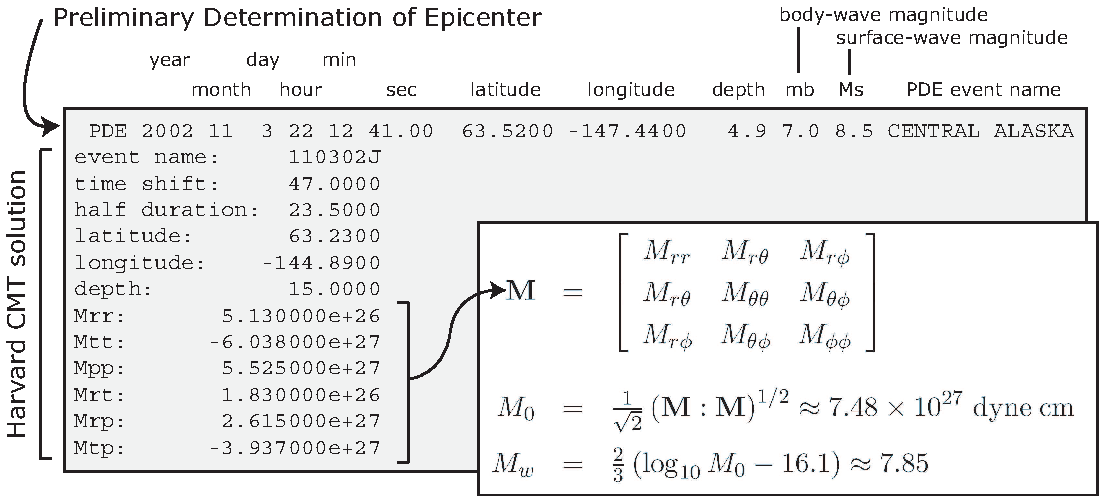
\includegraphics[width=1\textwidth]{figures/Denali_CMT.pdf}
\end{center}
\caption{\texttt{CMTSOLUTION} file obtained from the Global CMT catalog. The
top line is the initial estimate of the source, which is used as a
starting point for the CMT solution. \textbf{M} is the moment tensor,
$M_{0}${\small{} }is the seismic moment, and $M_{w}$ is the moment
magnitude.}
\label{fig:CMTSOLUTION-file}
\end{figure}
The \texttt{CMTSOLUTION} should be edited in the following way:

\begin{itemize}
\item For point-source simulations (see finite sources, page \pageref{To-simulate-a}),
setting the source half-duration parameter \texttt{half duration} equal to zero corresponds to simulating a step source-time
function (Heaviside), i.e., to using a moment-rate function that is a delta function. If
\texttt{half duration} is not set to zero, the code will use a smooth (pseudo) Heaviside source-time function
with a corresponding Gaussian moment-rate function
(i.e., a signal with a shape similar to a `smoothed triangle', as
explained in \citet{KoTr02a} and shown in Fig~\ref{fig:gauss.vs.triangle})
with half-width \texttt{half duration}.

Often, it is preferable to run the solver with \texttt{half duration} set to zero and convolve
the resulting synthetic seismograms in post-processing after the run,
because this way it is easy to use a variety of source-time functions
(see Section \ref{sec:Process-data-and-syn}). \citet{KoTr02a} determined
that the noise generated in the simulation by using a step source
time function may be safely filtered out afterward based upon a convolution
with the desired source-time function and/or low-pass filtering. Use
the postprocessing script \texttt{process\_syn.pl} (see Section \ref{sub:process_syn.pl})
with the \texttt{-h} flag, or the serial code \texttt{convolve\_source\_timefunction.f90}
and the script \texttt{utils/convolve\_source\_timefunction.csh} for
this purpose, or alternatively use signal-processing software packages
such as \href{http://www.iris.edu/software/sac/}{SAC}. Type
\begin{verbatim}
make convolve_source_timefunction
\end{verbatim}
to compile the code and then set the parameter \texttt{hdur} in \texttt{utils/convolve\_source\_timefunction.csh}
to the desired half-duration.

\item To use a monochromatic source-time function instead, enable the flag \texttt{USE\_MONOCHROMATIC\_CMT\_SOURCE} in \texttt{Par\_file}. In this case, \texttt{half
duration} will be interpreted as the period of the source-time function. By default, the left side of the source-time function is applied with a Hanning taper at a length of 200.0~s. This can be configured through \texttt{TAPER\_MONOCHROMATIC\_SOURCE} in \texttt{constants.h} file.

\item The zero time of the simulation corresponds to the center of the triangle/Gaussian,
or the centroid time of the earthquake. The start time of the simulation
is $t=-1.5*\texttt{half duration}$ (the 1.5 is to make sure the moment-rate function is very close to zero
when starting the simulation. This avoids spurious high-frequency oscillations).
To convert to absolute time $t_{\mathrm{abs}}$, set

\begin{lyxcode}
$t_{\mathrm{abs}}=t_{\mathrm{pde}}+\texttt{time shift}+t_{\mathrm{synthetic}}$
\end{lyxcode}
where $t_{\mathrm{pde}}$ is the time given in the first line of the
\texttt{CMTSOLUTION}, \texttt{time shift} is the corresponding value
from the original \texttt{CMTSOLUTION} file and $t_{\mathrm{synthetic}}$
is the time in the first column of the output seismogram.

\end{itemize}
%
\begin{figure}
\noindent \begin{centering}
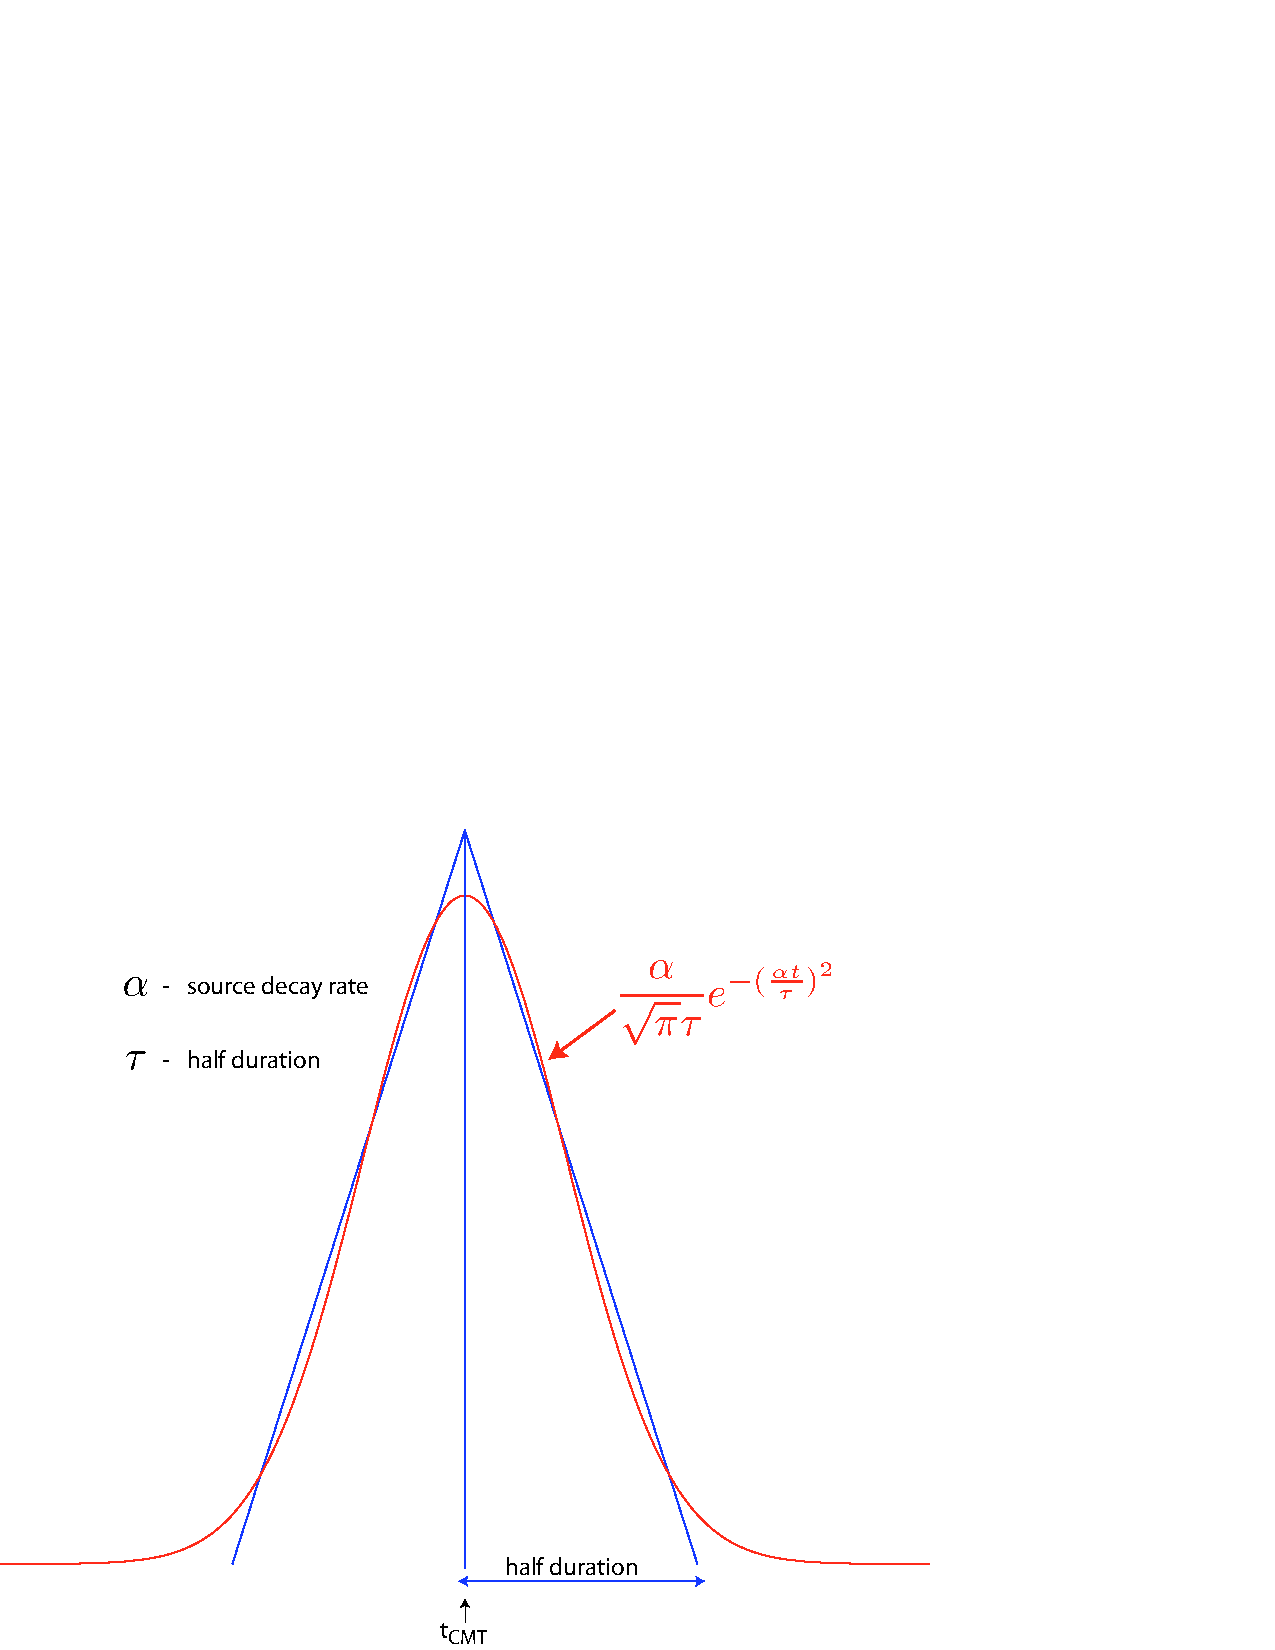
\includegraphics[width=3in]{figures/gauss_vs_triangle_mod.pdf}
\par\end{centering}
\caption{Comparison of the shape of a triangle and the Gaussian function actually used.}
\label{fig:gauss.vs.triangle}
\end{figure}

If you know the earthquake source in strike/dip/rake format rather than in \texttt{CMTSOLUTION} format,
use the C code \texttt{utils/strike\_dip\_rake\_to\_CMTSOLUTION.c} to convert it.
The conversion formulas are given for instance in \cite{AkRi80}.
Note that the \cite{AkRi80} convention is slightly different from the Global/Harvard \texttt{CMTSOLUTION} convention
(the sign of some components is different). The C code outputs both.\newline


Centroid latitude and longitude should be provided in geographical
coordinates. The code converts these coordinates to geocentric coordinates~\citep{DaTr98}.
Of course you may provide your own source representations by designing
your own \texttt{CMTSOLUTION} file. Just make sure that the resulting
file adheres to the Global/Harvard CMT conventions (see Appendix~\ref{cha:Reference-Frame-Convention}).
Note that the first line in the \texttt{CMTSOLUTION} file is the Preliminary Determination of Earthquakes (PDE) solution performed by the USGS NEIC, which is used as a seed for the Global/Harvard CMT inversion. The PDE solution is based upon P waves and often gives the hypocenter of the earthquake, i.e., the rupture initiation point, whereas the CMT solution gives the `centroid location', which is the location with dominant moment release. The PDE solution is not used by our software package but must be present anyway in the first line of the file.\newline


In the current version of the code, the solver can run with a non-zero \texttt{time shift} in the \texttt{CMTSOLUTION} file. Thus one does not need to set \texttt{time shift} to zero as it was the case for previous versions of the code. \texttt{time shift} is only used for writing centroid time in the SAC headers (see Appendix~\ref{cha:SAC-headers}). CMT time is obtained by adding \texttt{time shift} to the PDE time given in the first line in the \texttt{CMTSOLUTION} file. Therefore it is recommended not to modify \texttt{time shift} to have the correct timing information in the SAC headers without any post-processing of seismograms.\newline


\label{To-simulate-a}To simulate a kinematic rupture, i.e., a finite-source
event, represented in terms of $N_{\mathrm{sources}}$ point sources,
provide a \texttt{CMTSOLUTION} file that has $N_{\mathrm{sources}}$
entries, one for each subevent (i.e., concatenate $N_{\mathrm{sources}}$
\texttt{CMTSOLUTION} files to a single \texttt{CMTSOLUTION} file).
At least one entry (not necessarily the first) must have a zero \texttt{time
shift}, and all the other entries must have non-negative \texttt{time
shift}. If none of the entries has a zero \texttt{time shift} in the \texttt{CMTSOLUTION} file, the smallest \texttt{time shift} is subtracted from all sources to initiate the simulation. Each subevent can have its own half duration, latitude, longitude,
depth, and moment tensor (effectively, the local moment-density tensor).\newline


Note that the zero in the synthetics does NOT represent the hypocentral
time or centroid time in general, but the timing of the \textit{center}
of the source triangle with zero \texttt{time shift} (Fig~\ref{fig:source_timing}).
%
\begin{figure}[htp]
\begin{centering}
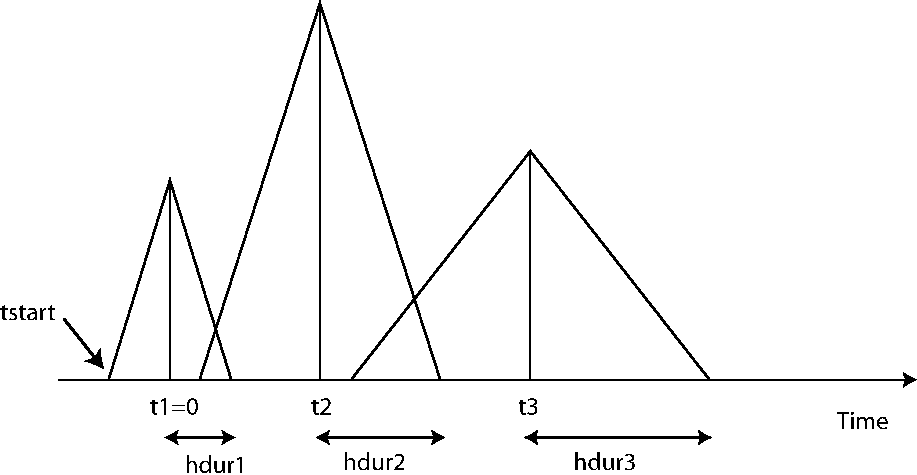
\includegraphics[width=5in]{figures/source_timing.pdf}
\end{centering}
%
\caption{Example of timing for three sources. The center of the first source
triangle is defined to be time zero. Note that this is NOT in general
the hypocentral time, or the start time of the source (marked as tstart).
The parameter \texttt{time shift} in the \texttt{CMTSOLUTION} file
would be t1(=0), t2, t3 in this case, and the parameter \texttt{half duration}
would be hdur1, hdur2, hdur3 for the sources 1, 2, 3 respectively.}
\label{fig:source_timing}
\end{figure}


Although it is convenient to think of each source as a triangle, in
the simulation they are actually Gaussians (as they have better frequency
characteristics). The relationship between the triangle and the Gaussian
used is shown in Fig~\ref{fig:gauss.vs.triangle}. For finite fault
simulations it is usually not advisable to use a zero half duration
and convolve afterwards, since the half duration is generally fixed
by the finite fault model.\newline

\vspace{1cm}

\noindent The \texttt{FORCESOLUTION} file should be edited in the
following way:
\begin{itemize}
\item The first line is only the header for the force solution, which can
be used as the identifier for the force source.
\item \texttt{time shift:} For a single force source, set
this  parameter equal to $0.0$ (The solver will not run otherwise!); the time
shift parameter would simply apply an overall time shift to the synthetics,
something that can be done in the post-processing (see Section \ref{sec:Process-data-and-syn}).
\item \texttt{half duration:} Set the half duration value (s) for step source-time
function. In case that the solver uses a (pseudo) Dirac delta source-time function to represent
a force point source, a very short duration of five time steps is automatically set by default.
For a Ricker source-time function, set the dominant frequency value (Hz).
See the parameter \texttt{source time function:} below for source-time functions.
\item \texttt{latitude:} Set the latitude of the force source.
\item \texttt{longitude:} Set the longitude of the force source.
\item \texttt{depth:} Set the depth of the force source (km).
\item \texttt{source time function:} Set the type of source-time function: 0 = Gaussian function, 1 = Ricker function, 2 = Heaviside (step) function, 3 = monochromatic function, 4 = Gaussian function as defined in \citet{Meschede2011}.
\item \texttt{factor force source:} Set the magnitude of the force source (units in Newton N).
\item \texttt{component dir vect source E:} Set the East component of a direction vector for the force
source. Direction vector is not necessarily a unit vector.
\item \texttt{component dir vect source N:} Set the North component of a direction vector for the force
source.
\item \texttt{component dir vect source Z\_up:} Set the vertical component of a direction vector for the force
source. Sign convention follows the positive upward direction.
\end{itemize}
\noindent Where necessary, set a \texttt{FORCESOLUTION} file in the
same way you configure a \texttt{CMTSOLUTION} file with $N_{\mathrm{sources}}$
entries, one for each subevent (i.e., concatenate $N_{\mathrm{sources}}$
\texttt{FORCESOLUTION} files to a single \texttt{FORCESOLUTION} file).
At least one entry (not necessarily the first) must have a zero \texttt{time
shift}, and all the other entries must have non-negative \texttt{time shift}.
Each subevent can have its own set of parameters \texttt{latitude}, \texttt{longitude}, \texttt{depth},
\texttt{half duration}, etc. \newline


\newpage
The solver can calculate seismograms at any number of stations for
basically the same numerical cost, so the user is encouraged to include
as many stations as conceivably useful in the \texttt{STATIONS} file,
which looks like this:
%
\begin{figure}[htp]
\begin{centering}
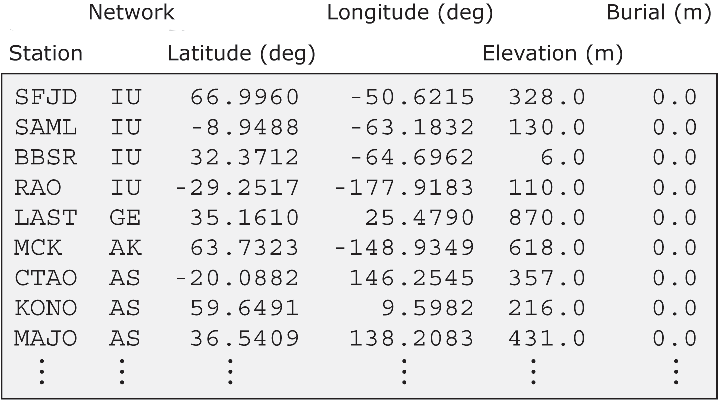
\includegraphics{figures/STATIONS_global_explained.pdf}
\end{centering}
%
\caption{Sample \texttt{STATIONS} file. Station latitude and longitude should
be provided in geographical coordinates. The width of the station
label should be no more than 32 characters (see \texttt{MAX\_LENGTH\_STATION\_NAME}
in the \texttt{constants.h} file), and the network label should be
no more than 8 characters (see \texttt{MAX\_LENGTH\_NETWORK\_NAME}
in the \texttt{constants.h} file).}
\end{figure}

Each line represents one station in the following format:
\begin{verbatim}
Station Network Latitude(degrees) Longitude(degrees) Elevation(m) burial(m)
\end{verbatim}
If you want to put a station on the ocean floor, just set
elevation and burial depth in the STATIONS file to 0.
Equivalently you can also set elevation to a negative value equal
to the ocean depth, and burial depth to 0.\newline


Solver output is provided in the \texttt{OUTPUT\_FILES} directory
in the \texttt{output\_solver.txt} file. Output can be directed to
the screen instead by uncommenting a line in \texttt{constants.h}:
{\small
\begin{verbatim}
! uncomment this to write messages to the screen
! integer, parameter :: IMAIN = ISTANDARD_OUTPUT
\end{verbatim}
}
Note that on very fast machines, writing to the screen may slow down
the code.\newline


While the solver is running, its progress may be tracked by monitoring
the `\texttt{timestamp{*}}' files in the \texttt{OUTPUT\_FILES} directory.
These tiny files look something like this:
{\small
\begin{verbatim}
Time step #           200
Time:    0.6956667      minutes
Elapsed time in seconds =     252.6748970000000
Elapsed time in hh:mm:ss =    0 h 04 m 12 s
Mean elapsed time per time step in seconds =     1.263374485000000
Max norm displacement vector U in solid in all slices (m) =    1.9325
Max non-dimensional potential Ufluid in fluid in all slices = 1.1058885E-22
\end{verbatim}
}
The \texttt{timestamp{*}} files provide the \texttt{Mean elapsed time
per time step in seconds}, which may be used to assess performance
on various machines (assuming you are the only user on a node), as
well as the
\texttt{Max norm displacement vector U in solid in all slices (m)}
and
\texttt{Max non-dimensional potential Ufluid in fluid in all slices}.
If something is wrong with the model, the mesh, or the source, you will see the
code become unstable through exponentionally growing values of the
displacement and/or fluid potential with time, and ultimately the
run will be terminated by the program when either of these values
becomes greater than \texttt{STABILITY\_THRESHOLD} defined in \texttt{constants.h}.
You can control the rate at which the timestamp files are written
based upon the parameter \texttt{NTSTEP\_BETWEEN\_OUTPUT\_INFO} in
the \texttt{Par\_file}.\newline


Having set the \texttt{Par\_file} parameters, and having provided
the \texttt{CMTSOLUTION} and \texttt{STATIONS} files, you are now
ready to launch the solver! This is most easily accomplished based
upon the \texttt{go\_solver} script (see Chapter~\ref{cha:Running-Scheduler}
for information about running the code through a scheduler, e.g.,
LSF). You may need to edit the last command at the end of the script
that invokes the \texttt{mpirun} command. Another option is to use
the \texttt{runall} script, which compiles and runs both mesher and
solver in sequence. This is a safe approach that ensures using the
correct combination of mesher output and solver input.\newline


It is important to realize that the CPU and memory requirements of
the solver are closely tied to choices about attenuation (\texttt{ATTENUATION})
and the nature of the model (i.e., isotropic models are cheaper than
anisotropic models). We encourage you to run a variety of simulations
with various flags turned on or off to develop a sense for what is
involved.\newline


For the same model, one can rerun the solver for different events
by simply changing the \texttt{CMTSOLUTION} file, and/or for different
stations by changing the \texttt{STATIONS} file. There is no need
to rerun the mesher. Of course it is best to include as many stations
as possible, since this does not add significantly to the cost of
the simulation.



\section{Note on the simultaneous simulation of several earthquakes}

\begin{figure}[H]
\begin{centering}
\includegraphics[width=2.2in]{figures/simultaneous_dir_struct.pdf}
\par\end{centering}
%
\caption{
Directory structure when simulating several earthquakes at once.
To improve readability, only directories have been drawn.}
\label{fig:simultaneous_dir_struct}
\end{figure}

Figure~\ref{fig:simultaneous_dir_struct} shows what the directory structure
should looks like when simulating multiple earthquakes at ones.

\begin{itemize}
\item The simulation is launched within the root directory \texttt{EXAMPLE\_ROOT\_DIR}\newline
(usually \texttt{mpirun -np N ./bin/xspecfem3D}).
\item \texttt{DATA} should contain the \texttt{Par\_file} parameter file with
\texttt{NUMBER\_OF\_SIMULTANEOUS\_RUNS} as explained in Chapter~\ref{cha:Running-the-Mesher}.
\item \texttt{DATABASES\_MPI} and {OUTPUT\_FILES} directory may contain the mesher output but they
are not required as they are superseded by the ones in the \texttt{runXXX} directories.
\item \texttt{runXXXX} directories must be created beforehand. There should be be as many as
\texttt{NUMBER\_OF\_SIMULTANEOUS\_RUNS} and the numbering should be contiguous, starting from \texttt{0001}.
They all should have \texttt{DATA},
\texttt{DATABASES\_MPI} and \texttt{OUTPUT\_FILES} directories. Additionally a \texttt{SEM} directory
containing adjoint sources have to be created to perform adjoint simulations.
\item \texttt{runXXXX/DATA} directories must all contain a \texttt{CMTSOLUTION} file,
a \texttt{STATIONS} file along with an eventual \texttt{STATIONS\_ADJOINT} file.
\item If \texttt{BROADCAST\_SAME\_MESH\_AND\_MODEL} is set to \texttt{.true.} in \texttt{DATA/Par\_file},
only \texttt{run0001/OUTPUT\_FILES} and \texttt{run0001/DATABASES\_MPI} directories need to contain the files
outputted by the mesher.
\item If \texttt{BROADCAST\_SAME\_MESH\_AND\_MODEL} is set to \texttt{.false.} in \texttt{DATA/Par\_file},
every \texttt{runXXXX/OUTPUT\_FILES} and \texttt{runXXXX/DATABASES\_MPI} directories need to contain the files
outputted by the mesher. Note that while the meshes might have been created from different models and
parameter sets, they should have been created using the same number of MPI processes.
\end{itemize}



